
\begin{figure}
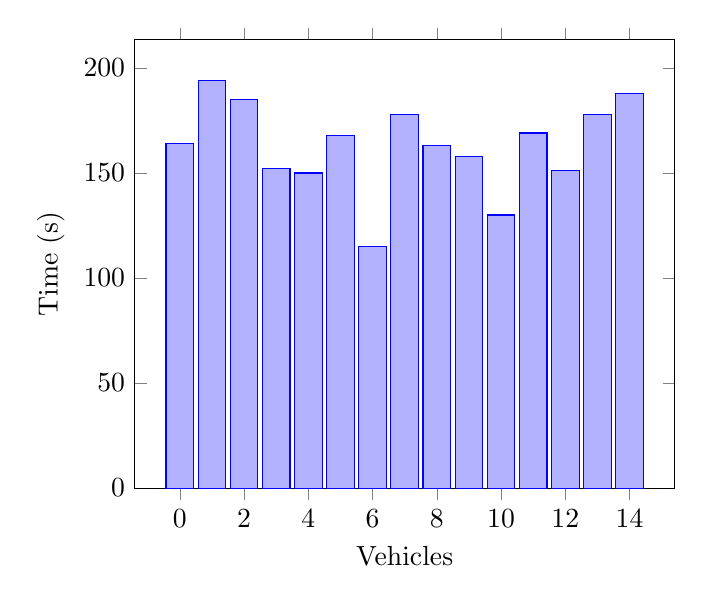
\begin{tikzpicture}
\begin{axis}[
legend style={anchor=west},
xlabel=Vehicles,
ylabel=Time (s),
ymin=0,
ybar,
]
\addplot coordinates {
(0, 164)
(1, 194)
(2, 185)
(3, 152)
(4, 150)
(5, 168)
(6, 115)
(7, 178)
(8, 163)
(9, 158)
(10, 130)
(11, 169)
(12, 151)
(13, 178)
(14, 188)
};

\end{axis}
\end{tikzpicture}
\label{tik:0:21_V, 20_V, 17_N, 15_S, 15_S.-30, 13_N, 13_N.-40, 11_N, 8_N, 7_N, 7_N.-60, 5_N, 4_N, 4_N.-60, 2_V}
\caption{0 percent diving with GSC on route $21_V, 20_V, 17_N, 15_S, 15_S.-30, 13_N, 13_N.-40, 11_N, 8_N, 7_N, 7_N.-60, 5_N, 4_N, 4_N.-60, 2_V$}
\end{figure}
